% This file was created with tikzplotlib v0.10.1.
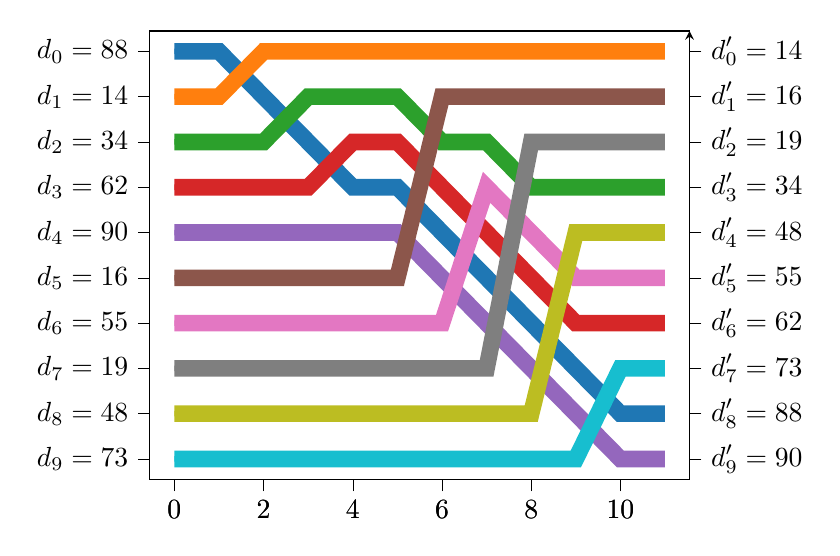
\begin{tikzpicture}

\definecolor{crimson2143940}{RGB}{214,39,40}
\definecolor{darkgray176}{RGB}{176,176,176}
\definecolor{darkorange25512714}{RGB}{255,127,14}
\definecolor{darkturquoise23190207}{RGB}{23,190,207}
\definecolor{forestgreen4416044}{RGB}{44,160,44}
\definecolor{goldenrod18818934}{RGB}{188,189,34}
\definecolor{gray127}{RGB}{127,127,127}
\definecolor{mediumpurple148103189}{RGB}{148,103,189}
\definecolor{orchid227119194}{RGB}{227,119,194}
\definecolor{sienna1408675}{RGB}{140,86,75}
\definecolor{steelblue31119180}{RGB}{31,119,180}

\begin{axis}[
tick align=outside,
tick pos=left,
x grid style={darkgray176},
xmin=-0.55, xmax=11.55,
xtick style={color=black},
y grid style={darkgray176},
ymin=-9.45, ymax=0.45,
ytick style={color=black},
ytick={0,-1,-2,-3,-4,-5,-6,-7,-8,-9},
yticklabels={
  \(\displaystyle d_0 = 88\),
  \(\displaystyle d_1 = 14\),
  \(\displaystyle d_2 = 34\),
  \(\displaystyle d_3 = 62\),
  \(\displaystyle d_4 = 90\),
  \(\displaystyle d_5 = 16\),
  \(\displaystyle d_6 = 55\),
  \(\displaystyle d_7 = 19\),
  \(\displaystyle d_8 = 48\),
  \(\displaystyle d_9 = 73\)
}
]
\addplot [line width=2pt, steelblue31119180]
table {%
0 0
1 0
2 -1
3 -2
4 -3
5 -3
6 -4
7 -5
8 -6
9 -7
10 -8
11 -8
};
\addplot [line width=2pt, darkorange25512714]
table {%
0 -1
1 -1
2 0
3 0
4 0
5 0
6 0
7 0
8 0
9 0
10 0
11 0
};
\addplot [line width=2pt, forestgreen4416044]
table {%
0 -2
1 -2
2 -2
3 -1
4 -1
5 -1
6 -2
7 -2
8 -3
9 -3
10 -3
11 -3
};
\addplot [line width=2pt, crimson2143940]
table {%
0 -3
1 -3
2 -3
3 -3
4 -2
5 -2
6 -3
7 -4
8 -5
9 -6
10 -6
11 -6
};
\addplot [line width=2pt, mediumpurple148103189]
table {%
0 -4
1 -4
2 -4
3 -4
4 -4
5 -4
6 -5
7 -6
8 -7
9 -8
10 -9
11 -9
};
\addplot [line width=2pt, sienna1408675]
table {%
0 -5
1 -5
2 -5
3 -5
4 -5
5 -5
6 -1
7 -1
8 -1
9 -1
10 -1
11 -1
};
\addplot [line width=2pt, orchid227119194]
table {%
0 -6
1 -6
2 -6
3 -6
4 -6
5 -6
6 -6
7 -3
8 -4
9 -5
10 -5
11 -5
};
\addplot [line width=2pt, gray127]
table {%
0 -7
1 -7
2 -7
3 -7
4 -7
5 -7
6 -7
7 -7
8 -2
9 -2
10 -2
11 -2
};
\addplot [line width=2pt, goldenrod18818934]
table {%
0 -8
1 -8
2 -8
3 -8
4 -8
5 -8
6 -8
7 -8
8 -8
9 -4
10 -4
11 -4
};
\addplot [line width=2pt, darkturquoise23190207]
table {%
0 -9
1 -9
2 -9
3 -9
4 -9
5 -9
6 -9
7 -9
8 -9
9 -9
10 -7
11 -7
};
\end{axis}

\begin{axis}[
axis y line=right,
tick align=outside,
x grid style={darkgray176},
xmin=-0.55, xmax=11.55,
xtick pos=left,
xtick style={color=black},
y grid style={darkgray176},
ymin=-9.45, ymax=0.45,
ytick pos=right,
ytick style={color=black},
ytick={0,-1,-2,-3,-4,-5,-6,-7,-8,-9},
yticklabel style={anchor=west},
yticklabels={
  \(\displaystyle d_0' = 14\),
  \(\displaystyle d_1' = 16\),
  \(\displaystyle d_2' = 19\),
  \(\displaystyle d_3' = 34\),
  \(\displaystyle d_4' = 48\),
  \(\displaystyle d_5' = 55\),
  \(\displaystyle d_6' = 62\),
  \(\displaystyle d_7' = 73\),
  \(\displaystyle d_8' = 88\),
  \(\displaystyle d_9' = 90\)
}
]
\addplot [line width=6pt, steelblue31119180]
table {%
0 0
1 0
2 -1
3 -2
4 -3
5 -3
6 -4
7 -5
8 -6
9 -7
10 -8
11 -8
};
\addplot [line width=6pt, darkorange25512714]
table {%
0 -1
1 -1
2 0
3 0
4 0
5 0
6 0
7 0
8 0
9 0
10 0
11 0
};
\addplot [line width=6pt, forestgreen4416044]
table {%
0 -2
1 -2
2 -2
3 -1
4 -1
5 -1
6 -2
7 -2
8 -3
9 -3
10 -3
11 -3
};
\addplot [line width=6pt, crimson2143940]
table {%
0 -3
1 -3
2 -3
3 -3
4 -2
5 -2
6 -3
7 -4
8 -5
9 -6
10 -6
11 -6
};
\addplot [line width=6pt, mediumpurple148103189]
table {%
0 -4
1 -4
2 -4
3 -4
4 -4
5 -4
6 -5
7 -6
8 -7
9 -8
10 -9
11 -9
};
\addplot [line width=6pt, sienna1408675]
table {%
0 -5
1 -5
2 -5
3 -5
4 -5
5 -5
6 -1
7 -1
8 -1
9 -1
10 -1
11 -1
};
\addplot [line width=6pt, orchid227119194]
table {%
0 -6
1 -6
2 -6
3 -6
4 -6
5 -6
6 -6
7 -3
8 -4
9 -5
10 -5
11 -5
};
\addplot [line width=6pt, gray127]
table {%
0 -7
1 -7
2 -7
3 -7
4 -7
5 -7
6 -7
7 -7
8 -2
9 -2
10 -2
11 -2
};
\addplot [line width=6pt, goldenrod18818934]
table {%
0 -8
1 -8
2 -8
3 -8
4 -8
5 -8
6 -8
7 -8
8 -8
9 -4
10 -4
11 -4
};
\addplot [line width=6pt, darkturquoise23190207]
table {%
0 -9
1 -9
2 -9
3 -9
4 -9
5 -9
6 -9
7 -9
8 -9
9 -9
10 -7
11 -7
};
\end{axis}

\end{tikzpicture}
